% Documentation for mlburg

\documentclass[11pt]{article}

\usepackage{graphicx}
\usepackage{url}
\usepackage{code}

\begin{document}
\parskip 10pt
\parindent 0in

\newcommand{\mlburg}{ML-Burg}
\newcommand{\burmgen}{\cd{BurmGen}}
\newcommand{\figureRef}[1]{\mbox{Figure\ \ref{#1}}}


\title{\mlburg\ --- Documentation}
\author{\begin{tabular}[t]{c@{\extracolsep{4em}}c}
\ \\
Florent Guillaume		&  Lal George			\\
\ \\	
 \'Ecole Normale Sup\'erieure	&  Room 2A-426			\\
 45, rue d'Ulm			&  AT\&T Bell Laboratories	\\
 75005 Paris, France		&  Murray Hill, NJ 07922	\\
\url{Florent.Guillaume@ens.fr} &  \url{george@research.att.com}
\end{tabular}}
\date{June 23, 1993}
\maketitle
\begin{center}
\copyright 1993 L. George, F. Guillaume.
\end{center}

		\section{Introduction}

\mlburg\ is a Standard ML version of the \cd{iburg}
tool developed by Fraser, Hanson and
Proebsting \cite{fraser-hanson-proebsting-92}. \mlburg\ generates
a Standard ML program to perform bottom-up rewriting of an input tree.
Cost information associated with each rewrite rule is used to derive
the minimum rewrite cost for the entire tree. A successful reduction
corresponds to rewriting the input tree to a special non-terminal
symbol called the {\em start non-terminal}. Upon successful reduction,
facilities are provided to walk the tree emitting semantic actions
corresponding to the rules that matched.

Like \cd{iburg}, \mlburg\ generates a program that consists of a
large case statement. Indeed, the \cd{i} in \cd{iburg} was meant to
indicate \mbox{{\em interpreted-}burg} to distinguish it from 
table driven implementations of similar
tools \cite{balachandran-dhamdhere-biswas-90,proebsting-pldi92}.
We arbitrarily decided to drop the \cd{i} (no pun intended).

Given a system of rewrite rules augmented with costs, called the {\em
\mlburg\ specification}, \mlburg\ generates the following:

\begin{itemize}
	\item\cd{signature BURM_INPUT_SPEC}
	\item\cd{signature BURM}
	\item\cd{structure BurmOps}
	\item\cd{functor BurmGen(In : BURM_INPUT_SPEC) : BURM}
\end{itemize}

The signature \cd{BURM_INPUT_SPEC} specifies utilities over the 
user supplied input
tree. The required matcher is obtained by applying the functor
\cd{BurmGen} to a structure matching \cd{BURM_INPUT_SPEC}.



		\section{ML-Burg specifications}

\figureRef{f:specification} shows the extended BNF grammar for 
\mlburg\ specifications. Grammar symbols are {\it italicized}, terminals
are in {\tt typewriter} font, \{{\it X}\} represents zero or more
occurrences of {\it X}, {\rm [}{\it X}{\rm ]} means {\it X} is optional, 
{\sl cost} is a non-negative integer, {\sl trailer} and {\sl header}
are arbitrary pieces of text, and everything else is an identifier.
An identifier is a leading alphabet followed by zero or more
alphanumeric characters and underscores. Comments are delimited
by {\tt (*}, and {\tt *)}. 

A specification consists of three parts: {\it declaration}, {\it rule},
and {\sl trailer}, separated by \verb|%%|.



\begin{figure}[t]
\small
 \begin{center}
 \sl
 \begin{tabular}{lcl}
   spec	& $\rightarrow$ &  {\it declaration}
		   	   \verb.%%. \{{\it rule}\}
			   \verb.%%. trailer				\\[1ex]

   {\it declaration} 
	& $\rightarrow$ & {\tt \%term} {\it op} \{\verb.|. {\it op}\}	\\
    	& $\mid$	& {\tt \%start} nonterminal			\\
	& $\mid$	& {\tt \%termprefix} termprefix			\\
	& $\mid$	& {\tt \%ruleprefix} ruleprefix			\\
	& $\mid$	& {\tt \%sig} signame				\\
	& $\mid$	& \verb.%{. header \verb.%}.			\\[1ex]

   {\it op}
	& $\rightarrow$ & operator {\rm [}{\tt =} opname{\rm ]}		\\[1ex]

   {\it rule}
	& $\rightarrow$ & nonterminal \verb.:. {\it tree} \verb.=. 
			  rulename {\rm [}{\tt (~}cost{\tt ~)}{\rm ]} 
			  \verb.;.					\\[1ex]

   {\it tree}
	& $\rightarrow$ & nonterminal					\\[1ex]
	& $\mid$	& operator {\rm [}{\tt (}
			  {\it tree}\{\verb.,.{\it tree}\}{\tt ~)}{\rm ]}
 \end{tabular}
 \end{center}
\caption{EBNF \mlburg\ specifications}

\label{f:specification}
\end{figure}

A {\tt \%term} declaration enumerates the operators or function symbols
used to construct nodes of the tree.  There must be at least one {\tt
\%term} declaration for a valid specification.  The {\tt \%start}
declaration, which defaults to the left hand side {\sl nonterminal} of the
first rule, declares the {\em start non-terminal}. The {\sl header} part is
text that is included verbatim at the beginning of the matcher.  The names
of the modules generated by \mlburg\ may be changed by using a {\tt
\%sig} declaration (case of {\sl signame} is not significant).  For example
if we had a line ``\verb.%sig glop.'' in the declarations, the generated
names would be {\tt GlopOps}, {\tt GLOP\_INPUT\_SPEC}, {\tt GLOP} and {\tt
GlopGen}.  This allows for multiple matchers in the same program.

\begin{figure}
\small
\begin{centercode}
%term ASGNI | ADDI | CVCI | INDIRC | I0I | ADDRLP | CNSTI
%termprefix T_
%start stmt
%%
stmt:   ASGNI(disp,reg)         = stmt_ASGNI_disp_reg   (1);
stmt:   reg                     = stmt_reg;
reg:    ADDI(reg,rc)            = reg_ADDI_reg_rc       (1);
reg:    CVCI(INDIRC(disp))      = reg_CVCI_INDIRC_disp  (1);
reg:    I0I                     = reg_I0I;
reg:    disp                    = reg_disp              (1);
disp:   ADDI(reg,con)           = disp_ADDI_reg_con;
disp:   ADDRLP                  = disp_ADDRLP;
rc:     con                     = rc_con;
rc:     reg                     = rc_reg;
con:    CNSTI                   = con_CNSTI;
con:    I0I                     = con_I0I;
%%
\end{centercode}
 \caption{Example of \mlburg\ specification.}
 \label{f:ex_spec}
\end{figure}

The rule-part of the specification (following the first {\tt \%\%})
describes the tree grammar or the rewrite rule system to use. The 
\mbox{{\sl nonterminal} {\tt :} {\it tree}} specification can be viewed a
rewrite rule of the form, \mbox{{\sl nonterminal} $\leftarrow$ {\it tree}}.
Each {\sl operator} used in a tree must be mentioned in a {\tt
\%term} declaration. The special case of \mbox{\sl nonterminal
$\leftarrow$ nonterminal}, specifies a chain rule. Associated with
each rule is an optional cost that defaults to zero. The {\sl
rulename}, which is not necessarily unique, is used to identify the
rule during the emission of semantic actions. It is important to note
that the same {\sl rulename} may be associated with multiple rules.

The {\sl trailer} is an arbitrary piece of text that is inserted at
the end of the generated matcher. This is typically segments of
program that will perform the semantic actions.

\figureRef{f:ex_spec} show a sample specification taken from
\cite{fraser-hanson-proebsting-92}. The {\tt \%termprefix}, and {\tt
\%ruleprefix} are explained in subsequent sections.


		\section{Interface between the matcher and the program}

	\subsection{structure BurmOps}

The \cd{structure BurmOps} declares a type \cd{ops} that enumerates
the operators or functions symbols specified in {\tt \%term}
declarations of the specification. The matcher cannot extract the
operator from the user supplied tree, or establish a correspondence
between nodes in the tree and operators in the specification.

In the example above (\figureRef{f:ex_spec}), the user may have
defined the tree to be:
\begin{code}
    datatype tree = ...
                  | CNSTI of int
                  ...
\end{code}
The data constructor \cd{CNSTI} is of arity 1, whereas, in the
specification it is used with arity 0.

For the example, the generated structure would be:

\begin{code}
    structure BurmOps = struct
      datatype ops = 
           T_ASGNI 
         | T_ADDI   
         | T_CVCI 
         | T_INDIRC
         | T_I0I   
         | T_ADDRLP 
         | T_CNSTI
    end
\end{code}

The {\tt \%termprefix}, if specified, is used to prepend the {\sl
termprefix} to each operator. If the optional {\sl {\tt =}opname} is
specified with the operator, then {\sl opname} is used in the
datatype \cd{ops} instead of the operator.

	\subsection{signature BURM\_INPUT\_SPEC}

The \cd{signature BURM_INPUT_SPEC}, shown below, specifies the
interface to the user supplied input tree.
\begin{code}
    signature BURM_INPUT_SPEC = sig
      type tree
      val opchildren : tree -> BurmOps.ops * (tree list)
    end
\end{code}
It contains:
\begin{itemize}
 \item The type {\tt tree} of trees on which the program operates.

 \item A function {\tt opchildren} which takes a {\tt tree} and returns the
operator (of type {\tt BurmOps.ops}) at the root of this tree, and a list
of children of this root (a {\tt tree list}). 
\end{itemize}

The function {\tt opchildren} must return the children in the order in
which they appear in the rules (which is the only order the matcher knows
of).  For example, if the root of the tree corresponds to the operator {\tt
ASGNI} (\figureRef{f:ex_spec}, the first element of the list
must be the tree corresponding to {\tt disp}, and the second 
to {\tt reg}.



	\subsection{signature BURM}

The structure generated by the functor \cd{BurmGen} matches the
signature \cd{BURM}. Specified in \cd{BURM} are:

\begin{itemize}
 	\item An exception \cd{NoMatch}, which is raised if \cd{reduce} is
called on a tree which cannot be rewritten to the start non-terminal.

 	\item The type \cd{tree} (the one passed to the functor).

 	\item A datatype \cd{rule} enumerating the rules of the tree
grammar. This datatype is defined by prepending to each {\sl rulename},
the {\sl ruleprefix} from a \cd{ruleprefix} declaration (if any).
The arity of each constructor is equal to the number of non-terminal
symbols in the pattern. Each \cd{(rule,tree)} pair specifies the
\cd{rule} and the \cd{tree} that matched each non-terminal symbol.
These pairs describe the remaining steps in the reduction. 

	 \item A function \cd{reduce} which takes a \cd{tree} and
returns a pair \verb|(rule * tree)|. As described above, the \cd{rule}
describes the best match that generated the start non-terminal, and the
\cd{tree} is the original input tree.
\end{itemize}

In the example above, the signature \cd{BURM} generated is:

\begin{centercode}
signature BURM = sig
  exception NoMatch
  type tree

  datatype rule = 
       stmt_ASGNI_disp_reg  of (rule*tree) * (rule*tree)
     | stmt_reg             of (rule*tree)
     | reg_ADDI_reg_rc      of (rule*tree) * (rule*tree)
     | reg_CVCI_INDIRC_disp of (rule*tree)
     | reg_I0I
     | reg_disp             of (rule*tree)
     | disp_ADDI_reg_con    of (rule*tree) * (rule*tree)
     | disp_ADDRLP
     | rc_con               of (rule*tree)
     | rc_reg               of (rule*tree)
     | con_CNSTI
     | con_I0I

  val reduce : tree -> (rule*tree)
end
\end{centercode}

The functions \cd{reduce} is used as follows: given a tree $t_0$,
\cd{reduce} returns an initial pair $(r_0, t_0)$ (it returns $t_0$ to
make the user program simpler - Section\ \ref{s:example}).
$r_0$
describes the first rule to apply to $t_0$ to perform the optimal
reduction.  This rule, except in trivial cases, will have in its
pattern several {\sl nonterminal}s which represent other trees to be
reduced.  To that end, the constructor $r_0$ carries the pairs 
\mbox{$(r_1,t_1), \ldots, (r_n,t_n)$} of its children.
$(r_i,t_i)$ corresponds to the $i$th {\sl nonterminal} in the tree pattern
for the rule $r_0$, when read from left to right.  These pairs can be used
to find the rule to use to reduce each child. In turn, the rules $r_1,
\ldots, r_n$ carry information about their children.

Why return the tree in addition to each rule?  Often, additional
information is stored in the tree, and it may be necessary to access this
information when a semantic action is executed. This information may
include constants like {\em integers}, {\em reals} or {\em string}, or more
complex objects like symbol table information.


		\section{Example}
		\label{s:example}

Using the \mlburg\ specification of \figureRef{f:ex_spec}, a sample
input to provide to the functor \cd{BurmGen} is shown below:
\begin{code}
      structure In : BURM_INPUT_SPEC = struct
	structure BO = BurmOps
	datatype tree = 
	      ASGNI  of tree * tree
	    | ADDI   of tree * tree
	    | CVCI   of tree
	    | INDIRC of tree
	    | I0I
	    | ADDRLP of string
	    | CNSTI  of int

	fun opchildren t =
	  case t of
	    ASGNI(t1,t2)  => (BO.T_ASGNI, [t1,t2])
	  | ADDI(t1,t2)   => (BO.T_ADDI,  [t1,t2])
	  | CVCI(t1)      => (BO.T_CVCI,  [t1])
	  | INDIRC(t1)    => (BO.T_INDIRC,[t1])
	  | I0I           => (BO.T_I0I,   [])
	  | ADDRLP _      => (BO.T_ADDRLP,[])
	  | CNSTI _       => (BO.T_CNSTI, [])
      end
\end{code}




In \figureRef{ex:prog} we show a sample function called \cd{walk} that
performs semantic actions. The semantic actions merely prints out the
rules that applied assuming the children of each node are traversed
from left to right. Note that in the action corresponding to the
\cd{reg_CVCI_INDIRC_disp} rule, the recursive call to \cd{walk},
specifically \cd{walk disp}, steps over the \cd{CVCI} and \cd{INDIRC}
nodes --- yet, information associated with the \cd{CVCI} or
\cd{INDIRC} is available to this rule.



\begin{figure}
\begin{centercode}
structure Example = struct 
  structure Burm = BurmGen (In)
  open In

  local val num = ref 1 in
    fun new s = (s^(makestring (!num)) before inc num)
  end

  fun walk (Burm.stmt_ASGNI_disp_reg (disp,reg), _) =
        let
          val (disp',reg') = (walk disp, walk reg)
          val stmt = new "stmt"
        in
          say (stmt^" <- ASGNI ("^disp'^" + "^reg'^")\\n"); stmt
        end
    ...
    | walk (Burm.reg_CVCI_INDIRC_disp disp, _) =
	let
	  val disp' = walk disp
	  val reg = new "reg"
	in
	  say (reg^" <- CVCI (INDIRC ("^disp'^"))\\n"); reg
	end
    ...
    | walk (Burm.con_CNSTI, CNSTI i) =
        let
          val con = new "con"
        in
          say (con^" <- CNSTI "^(makestring i)^"\\n"); con
        end
    ...
    | walk _ = (print "Error, bad match in walk\\n"; raise Match)


  fun doit t = walk (Burm.reduce t)

  val sampleTree = ASGNI (ADDRLP "p",
                          ADDI (CVCI (INDIRC (ADDRLP "c")),
                                CNSTI 4))
end
\end{centercode}
 \caption{Example program.}
 \label{ex:prog}
\end{figure}

A graphical representation of \cd{sampleTree} and the result of
executing: 
\begin{code}
    - open Example; doit sampleTree;
\end{code}
is shown in \figureRef{ex:output}.

\begin{figure}
  \begin{center}
    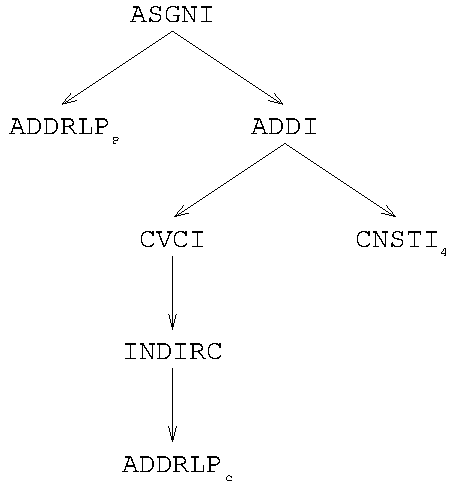
\includegraphics[width=3in]{tree}
  \end{center}%

\vskip 1in

\begin{centercode}
disp1 <- ADDRLP p
disp2 <- ADDRLP c
reg3 <- CVCI (INDIRC (disp2))
con4 <- CNSTI 4
disp5 <- ADDI (reg3,con4)
reg6 <- disp5
stmt7 <- ASGNI (disp1 + reg6)
\end{centercode}
 \caption{{\tt sampleTree} and the produced output.}
 \label{ex:output}
\end{figure}

	\section{Using {\tt mlburg} and debugging}

The executable for \mlburg\ is usually called \cd{mlburg}.  When \cd{mlburg} is
presented with a file name {\em filename}{\tt .burg}, a file {\em
filename}{\tt .sml} is created - assuming no errors were encountered. This
generated file will contain all the modules described above, and can be
directly loaded into an interactive session.  The error messages displayed
during the execution of \cd{mlburg} are self-explanatory.

During execution, a \cd{NoMatch} is raised when the tree cannot be reduced
to the start non-terminal.  For example, suppose that the function
\cd{reduce} was called on the tree \cd{CNSTI}.  Obviously, \cd{CNSTI} can
only be reduced to a \cd{con} and an \cd{rc}.  The matcher would then print
the message~:
\begin{code}
    No Match on nonterminal 0
    Possibilities were :
    rule 9 with cost 0
    rule 11 with cost 0
\end{code}
The {\sl nonterminal}s and rules are printed using integers, but a
correspondence between these integers and the identifiers used in the
specification can be found at the beginning of the generated SML file.

Note, however, that such debugging information will only be useful if the
incorrect match occurs at the first level of the reduction to the start
non-terminal.  If \cd{reduce} is called with \cd{ASGNI(I0I,\(x\))}, the
problem occurs deeper, because it is ultimately \cd{I0I} that cannot be
reduced to a \cd{disp}, and the fact that the whole tree cannot be reduced
to the start non-terminal is only a consequence of it.  In such cases, the
matcher will only give the message~:
\begin{code}
    No Match on nonterminal 0
    Possibilities were : 
\end{code}
At this stage it would be necessary to check the completeness of the
rewrite system. Automated tools to do this, may be expected in the
future\cite{emmelmann-92}. 

\bibliographystyle{acm}
\bibliography{doc}
\end{document}
